\chapter{Experiments}
\label{chapter:ch4}

Chapter 4 focuses on the experiments conducted to evaluate the effectiveness of our two-stage pre-training approach (Sec.~\ref{expTwoStage}). We provide detailed insights into the experimental setup. Furthermore, we present the experimental results that demonstrate the performance of our proposed method compared to the baseline. We conduct a comprehensive analysis of the results, discussing the strengths and limitations of our approach in detail. Subsequently, we explore the impact of changing the image encoder architecture (Sec.~\ref{expDiffImgEnc}), investigating how variations such as the use of different transformer models affect the overall performance. This analysis provides valuable insights into the generalization capabilities and adaptability of our method across different image encoders. Afterwards, we conduct a comprehensive comparison between our best-performing model and previous work methods (Sec.~\ref{expComparison}). By comparing our proposed method to previous approaches, we demonstrate that it brings significant advancements in integrating vision and language in the medical field. This highlights its effectiveness in addressing the challenges specific to medical applications. Finally, in Section~\ref{qualitativeResult}, we present the qualitative results of our model's performance on medical VQA. This analysis includes the presentation of successful cases and failure cases, and a comprehensive examination.

\section{Effectiveness of Two-stage Pre-training}\label{expTwoStage}
The purpose of the proposed two-stage pre-training method is to determine if it can achieve better results compared to the original single-stage approach. We also aim to highlight the importance of acquiring basic organ knowledge before the original pre-training stage. Through the evaluation of model performance with and without the initial stage, we can demonstrate the importance of having a robust foundation in organ understanding. This analysis enables us to demonstrate the value derived from incorporating knowledge of organs into the model's learning process.

% The findings also emphasize the significance of the order in which the pre-training stages are conducted, with the stage one followed by stage two proving to be crucial. Acquiring fundamental organ knowledge prior to the original pre-training stage is deemed essential. Furthermore, the results highlight that the original pre-training alone falls short in providing the necessary basic organ understanding to the model. These findings collectively reinforce the importance of incorporating the two-stage pre-training approach for improved performance and a stronger foundation in organ knowledge.

\subsection{Experimental Setup}\label{setup}

{\bf First Stage:} 
The first stage involves training on the CHAOS dataset \cite{kavur2021chaos} for image segmentation. We utilize ViT/16 \cite{dosovitskiy2020vit} pre-trained on CLIP \cite{radford2021learning} as the image encoder and RoBERTa \cite{zhuang-etal-2021-robustly} as the text encoder. The pre-training stage one takes approximately 3 hours on a single GPU A6000 with 48 GB memory. We use a batch size of 32 and an image size of 224. The epoch is set to 100, and we employ the Adam optimizer \cite{kingma2015adam} with a learning rate of 1e-4. 

{\bf Second Stage:} 
In the pre-training stage two, we use the MedICat \cite{subramanian-2020-medicat} and ROCO datasets \cite{Pelka2018RadiologyOI} for the original self-supervised pre-training technique. The image encoder and text encoder maintain consistency with the configuration employed in stage one. The pre-training stage two requires around 72 hours of training on four GPU A6000 with 48 GB memory each. The batch size and image size are consistent with stage one. We use the Adam  \cite{kingma2015adam} with a learning rate of 1e-5, a warm-up ratio of 10\%, and linear decay of the learning rate to 0 after 10\% of the total training steps. The epoch is set to 30. 

{\bf Fine-tuning:}
In the fine-tuning phase, we conduct experiments using the VQA SLAKE dataset \cite{liu2021slake}. The training process takes around 2 hours and is performed on a single GPU A6000 with 48 GB of memory. We utilize a batch size of 32 and set the image resolution to 384x384. The epoch is set to 15. We employ the Adam optimizer \cite{kingma2015adam} with a learning rate of 1e-6. To enhance the fine-tuning process, we apply RandAugment \cite{cubuk2020randaugment}, following previous work \cite{Dou_2022_CVPR}. The evaluation metric used is VQA classification accuracy, as shown in Equation~\ref{eq:vqa_acc}. We specifically analyze the performance in both closed-ended and open-ended categories. The implementation is based on the PyTorch \cite{paszke2017automatic} and Huggingface \cite{wolf2019huggingface} Transformers library.

\begin{equation}\label{eq:vqa_acc}
    Accuracy = {\frac{\#\ of\ correct\ answers}{\#\ of\ total\ questions}}
\end{equation}

\subsection{Results}\label{result1}

{\bf Comparing One-Stage and Two-Stage Pre-Training:} Table~\ref{tab:compareTwoStage} shows the performance comparison between one-stage pre-training and two-stage pre-training on VQA SLAKE test split. The results of the two-stage pre-training approach demonstrate its superiority over the original one-stage pre-training method by achieving a 1.6\% performance improvement. This highlights the necessity of employing the two-stage pre-training technique for medical datasets. 

\begin{table}[h]
    \centering
    \caption{Performance of one-stage pre-training framework vs proposed two-stage pre-training.}
    \setlength{\tabcolsep}{3.pt}
    \begin{tabular}{l c  c c c  c}
        \toprule
        Method &  Open-ended & Closed-ended & Overall  \\
        \midrule
        One-Stage Pre-training \cite{Dou_2022_CVPR}  & 79.3 & 85.1 & 81.5 \\
        \rowcolor{LightCyan}
        Two-Stage Pre-training & 80.5 & 87.0 & 83.1 \\
        \bottomrule
    \end{tabular}
    \label{tab:compareTwoStage}
\end{table}


{\bf Sequence of Pre-Training Stages:} Furthermore, we investigate the impact of switching the order of pre-training stages. Table~\ref{tab:compareOrder} illustrates the results, indicating that performing a second-stage pre-training followed by first-stage pre-training leads to a 0.5\% improvement compared to the baseline of one-stage pre-training. By employing the proposed pre-training step, the model achieved a performance enhancement of 1.6\%. This shows the significance of the pre-training order, indicating that conducting medical image segmentation as the first-step pre-training provides the model with organ-specific knowledge prior to the original pre-training is crucial.
%Comparison of performance with modified pre-training order.
%Performance of one-stage pre-training framework vs proposed two-stage pre-training.
\begin{table}[h]
    \centering
    \caption{Comparison of performance with modified pre-training order.}
    \setlength{\tabcolsep}{3.pt}
    \begin{tabular}{l c  c c c  c}
        \toprule
        Method &  Open-ended & Closed-ended & Overall  \\
        \midrule
         One-Stage Pre-training \cite{Dou_2022_CVPR}  & 79.3 & 85.1 & 81.5 \\
         $\nth{2} \; Stage \Rightarrow  \nth{1} \; Stage$  & 79.7 & 85.6 & 82.0 \\
        \rowcolor{LightCyan}
        $\nth{1} \; Stage \Rightarrow  \nth{2} \; Stage$ & 80.5 & 87.0 & 83.1 \\
        \bottomrule
    \end{tabular}
    \label{tab:compareOrder}
\end{table}


{\bf Pre-training Stage One's Effectiveness:} We also evaluate the effectiveness of pre-training stage one in isolation by excluding pre-training stage two. We conduct pre-training stage one alone and compare its performance with a model initialized with random weights. The results, presented in Table~\ref{tab:effectiveOfStageOne}, demonstrate a substantial 3.4\% improvement in performance compared to the random weight initialization approach. This indicates that pre-training stage one alone can effectively equip the model with valuable knowledge relevant to medical vision-language tasks.

\begin{table}[h]
    \centering
    \caption{Comparative performance analysis: Pre-training stage one vs. Random weights initialization}
    \setlength{\tabcolsep}{3.pt}
    \begin{tabular}{l c  c c c  c}
        \toprule
        Method &  Open-ended & Closed-ended & Overall  \\
        \midrule
        Random Weights & 78.2 & 76.0 & 77.3 \\
        \rowcolor{LightCyan}
        Pre-training Stage One & 79.1 & 83.2 & 80.7 \\
        \bottomrule
    \end{tabular}
    \label{tab:effectiveOfStageOne}
\end{table}

\section{Performance of Different Image Encoder Configurations}\label{expDiffImgEnc}
In the two-stage pre-training experiment, we conducted an investigation to assess the model's ability to generalize across different architecture designs by changing the image encoder from Vision-Transformer (ViT/16) \cite{dosovitskiy2020vit} to Swin Transformer \cite{Liu_2021_ICCV}. By evaluating the performance of the two-stage pre-training method with different image encoders, we aimed to investigate the generalization capability and adaptability of the model across distinct architecture choices. The implementation details are similar to Section~\ref{setup}

Table~\ref{tab:diffImageEncoder} shows the downstream performance results on the SLAKE test split using different image encoders. The Swin Transformer achieved a VQA accuracy of 81.4\% with original pre-training. However, when we applied the two-stage pre-training, the performance improvement was only 0.9\%. On the other hand, the ViT (Vision Transformer) exhibited a more notable improvement of 1.6\%. This suggests that the ViT (Vision Transformer) is more suitable for this specific method. We hypothesize that the lack of significant improvement with Swin Transformer could be attributed to its increased model complexity. Given the limited amount of medical images for training, the Swin Transformer may have been more prone to overfitting, leading to a smaller performance gain compared to ViT.

\begin{table}[h]
    \centering
    \caption{Comparative performance analysis: Different image encoder setting configurations}
    \setlength{\tabcolsep}{3.pt}
    \begin{tabular}{l c c c c}
        \toprule
        Method & Image Encoder & Open-ended & Closed-ended & Overall  \\
        \midrule
        One-stage Pre-training & Swin & 79.3 & 84.6 & 81.4 \\
        Two-stage Pre-training & Swin & 79.6 & 86.5 & 82.3 \\
        One-stage Pre-training & ViT & 79.3 & 85.1 & 81.5 \\
        \rowcolor{LightCyan}
        Two-stage Pre-training & ViT & 80.5 & 87.0 & 83.1 \\
        \bottomrule
    \end{tabular}
    \label{tab:diffImageEncoder}
\end{table}

\section{Comparison with Previous Works}\label{expComparison}
The purpose of our experiment was to evaluate the performance of our two-stage pre-training framework in comparison to several previous methods. By conducting this comparison, we aimed to assess the effectiveness and superiority of our proposed approach. The implementation details of our experiment were similar to those described in Section~\ref{setup}.

We classified the models into two groups: pre-trained models and non pre-trained models. The non pre-trained models included the baseline model from the SLAKE dataset \cite{liu2021slake}, while the pre-trained models consisted of PubMedCLIP \cite{eslami-etal-2023-pubmedclip} , METER \cite{Dou_2022_CVPR}, and ARL \cite{chen2022align}. 

As shown in Table~\ref{tab:compareWithPrevious}, our two-stage pre-training method demonstrated superior performance compared to the non pre-trained models (SLAKE baseline) by a significant margin. This finding highlights the crucial role of pre-training in vision-language tasks. Furthermore, our model outperformed pre-trained models that utilized a similar or smaller number of images during pre-training, such as PubMedCLIP and METER models. This showcases the effectiveness of our two-stage pre-training approach over the original one-stage pre-training method. However, our method was surpassed by ARL, which had access to a larger dataset of approximately 700K image-caption pairs during pre-training. This emphasizes the importance of the number of pre-trained images in achieving optimal results in the medical vision-language domain.

\begin{table}[h]
    \centering
    \caption{Comparative performance with previous works}
    \setlength{\tabcolsep}{3.pt}
    \begin{tabular}{l c c c c}
        \toprule
        Method & Pre-train Images & Open-ended & Closed-ended & Overall  \\
        \midrule
        SLAKE baseline \cite{liu2021slake}& 0 & 72.2 & 79.8 & 75.4 \\
        PubMedCLIP \cite{eslami-etal-2023-pubmedclip} & $\approx$80K & 78.4 & 82.5 & 80.1 \\
        METER \cite{Dou_2022_CVPR} & $\approx$300K & 79.3 & 85.1 & 81.5 \\
        Two-stage Pre-training & $\approx$300K & 80.5 & 87.0 & 83.1 \\
        \rowcolor{LightCyan}
        ARL \cite{chen2022align} & $\approx$700K & 81.9 & 91.4 & 85.6 \\
        \bottomrule
    \end{tabular}
    \label{tab:compareWithPrevious}
\end{table}

\section{Qualitative Examples} \label{qualitativeResult}
Figure~\ref{fig:qualitative1} to~\ref{fig:qualitative8} show the qualitative examples from our method on the SLAKE test splits. They display both successful cases and some failure cases. The qualitative results indicate that the model possesses knowledge about fundamental organ knowledge. For example, in Figure~\ref{fig:qualitative1}, the question is "Does the patient have liver cancer?" Our model can provide the correct answer, demonstrating its understanding of a healthy liver's appearance, which is crucial for accurate responses.

However, in Figure~\ref{fig:qualitative2}, we present a failure case where the question is "What diseases are included in the picture?" Our model provides an incorrect answer. Nonetheless, the model demonstrates knowledge of the abnormality's location when asked, "Where is/are the abnormality located?" and provides the correct answer. This indicates that the model possesses fundamental organ knowledge but lacks specific disease-related knowledge. This limitation can be attributed to the fact that in pre-training stage one, we focused only on semantic segmentation of organs and did not include disease-related information.

Additionally, the model exhibits some failure cases, as shown in Figure~\ref{fig:qualitative8}, particularly when processing abdomen images. For instance, when asked the question "Does the picture contain colon?" the model incorrectly responds. Similarly, when presented with the question "Which part of the human body is the organ located in this image?" the model mistakenly identifies it as the chest instead of the pelvic cavity. These failures can be attributed to the fact that the pre-training stage one does not include specific training on this particular body part. To address these shortcomings, one potential avenue for future improvement would involve augmenting the dataset used in pre-training stage one to encompass a wider range of organ and body part representations. By exposing the model to a more diverse set of examples, it is expected to develop a better understanding of various anatomical regions and improve its performance on related questions in the medical visual question answering task.

\begin{figure}[t]
\begin{center}
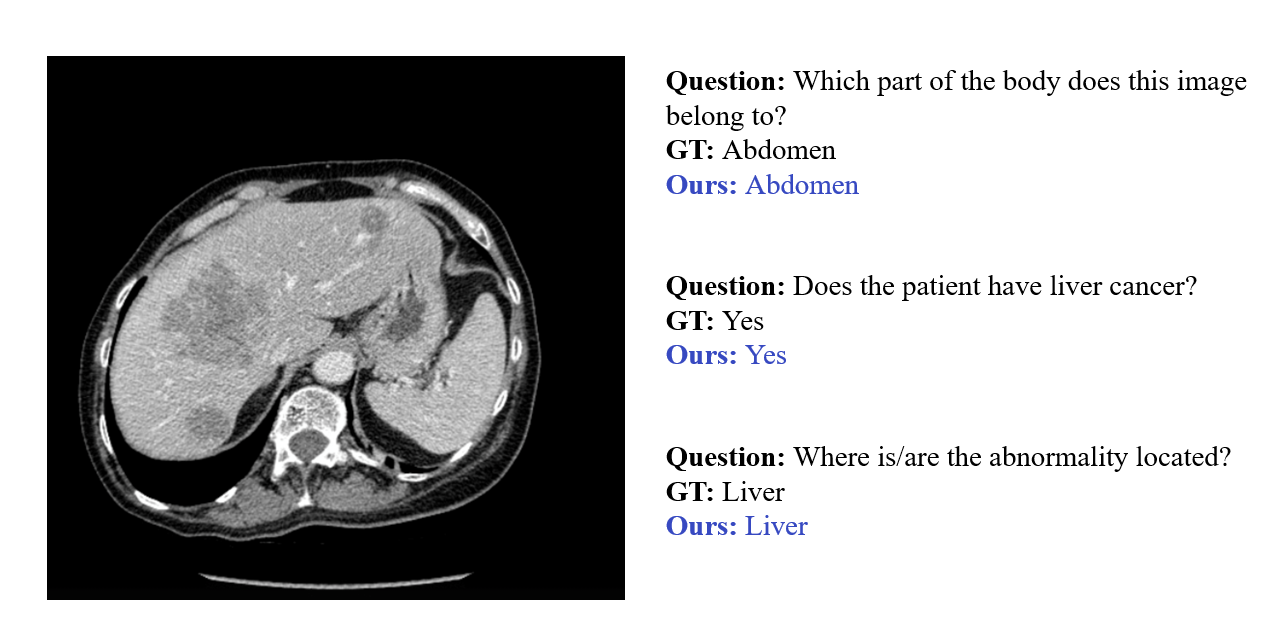
\includegraphics[width=1.0\linewidth]{Chapter_4/chap4_result1.png}
\end{center}
   \caption{Qualitative examples from our method on the SLAKE test splits.
}
\label{fig:qualitative1}
\end{figure}


\begin{figure}[t]
\begin{center}
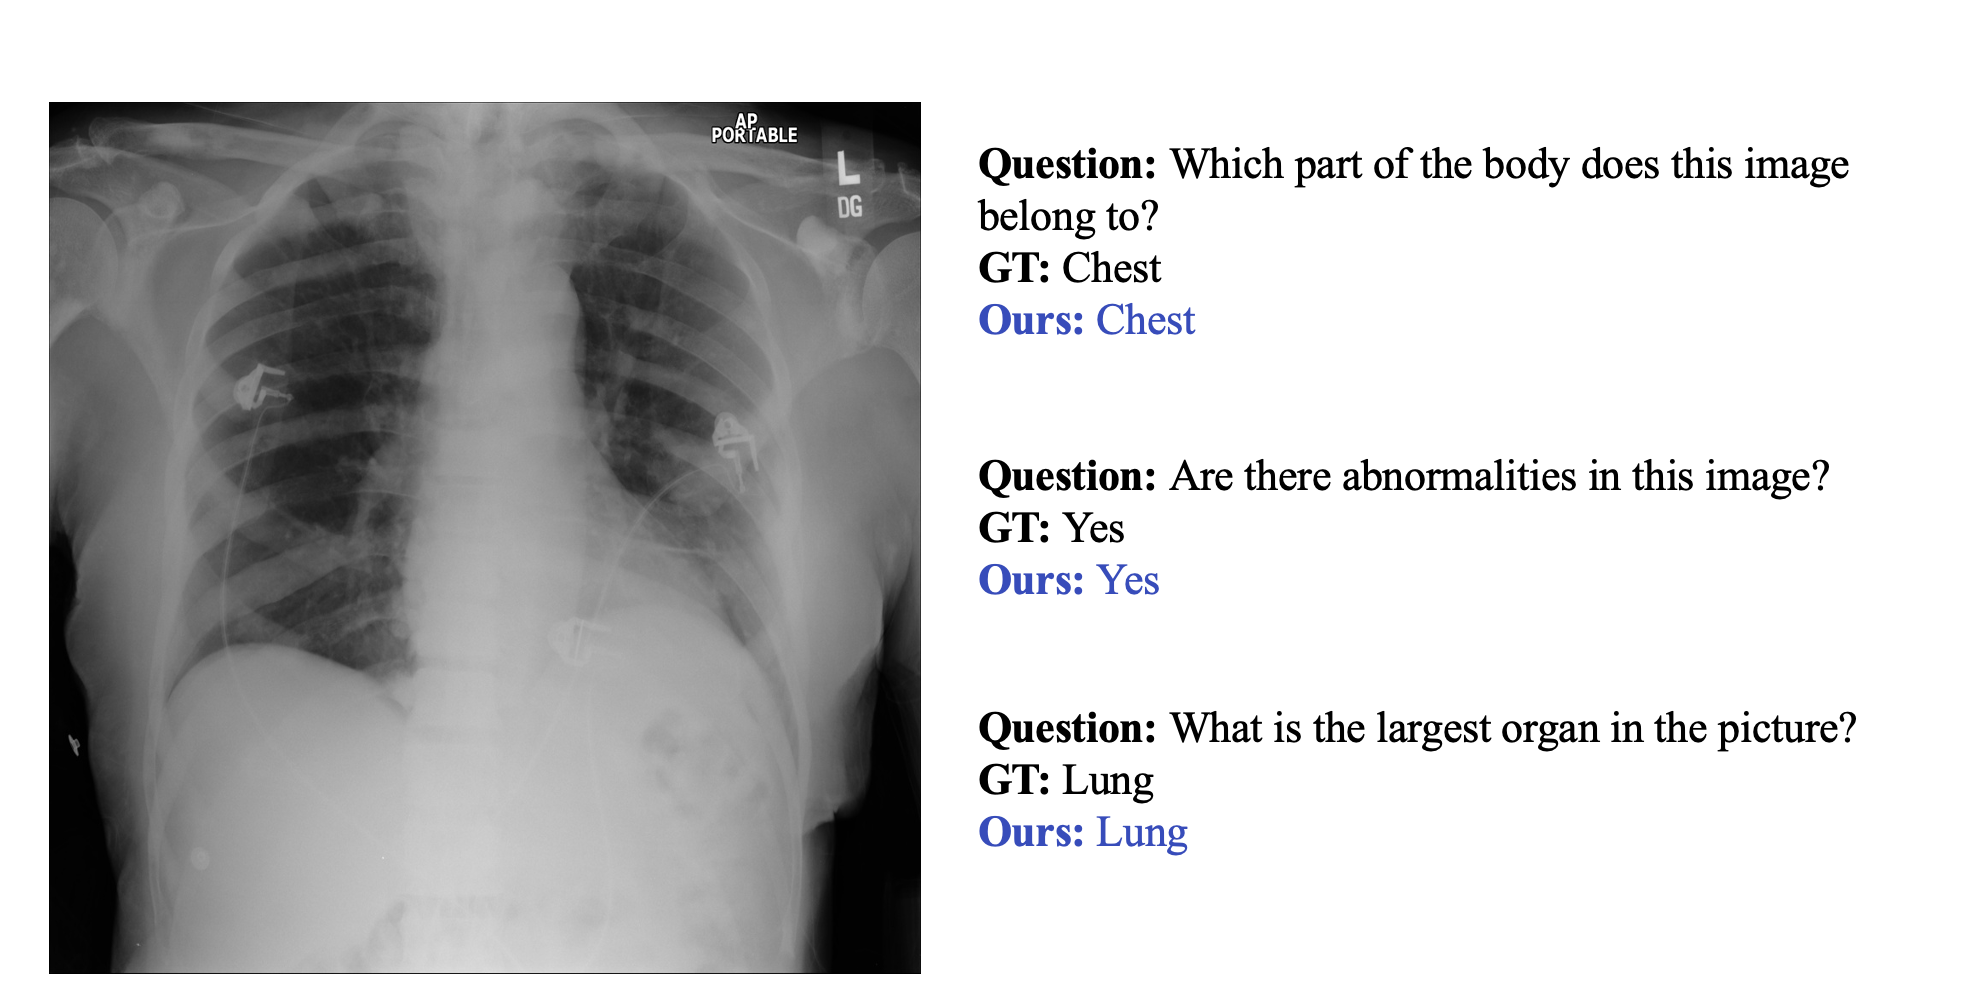
\includegraphics[width=1.0\linewidth]{Chapter_4/chap4_result3.png}
\end{center}
   \caption{Qualitative examples from our method on the SLAKE test splits.
}
\label{fig:qualitative3}
\end{figure}


\begin{figure}[t]
\begin{center}
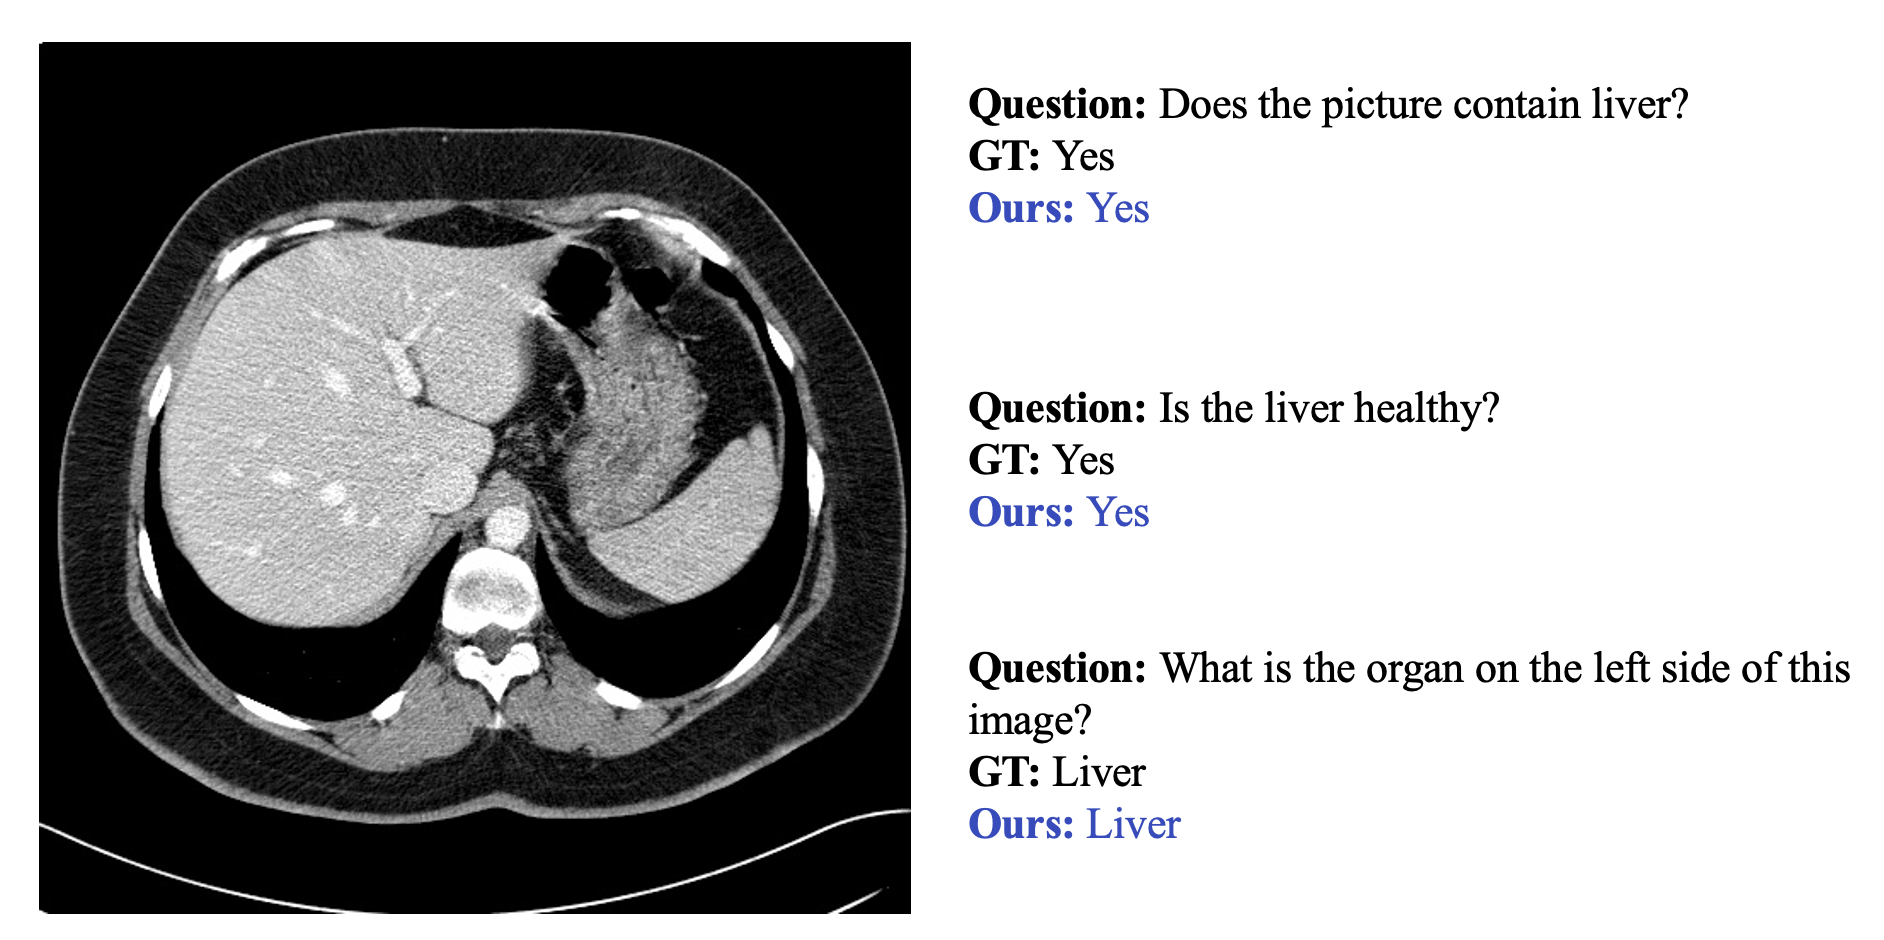
\includegraphics[width=1.0\linewidth]{Chapter_4/chap4_result4.png}
\end{center}
   \caption{Qualitative examples from our method on the SLAKE test splits.
}
\label{fig:qualitative4}
\end{figure}


\begin{figure}[t]
\begin{center}
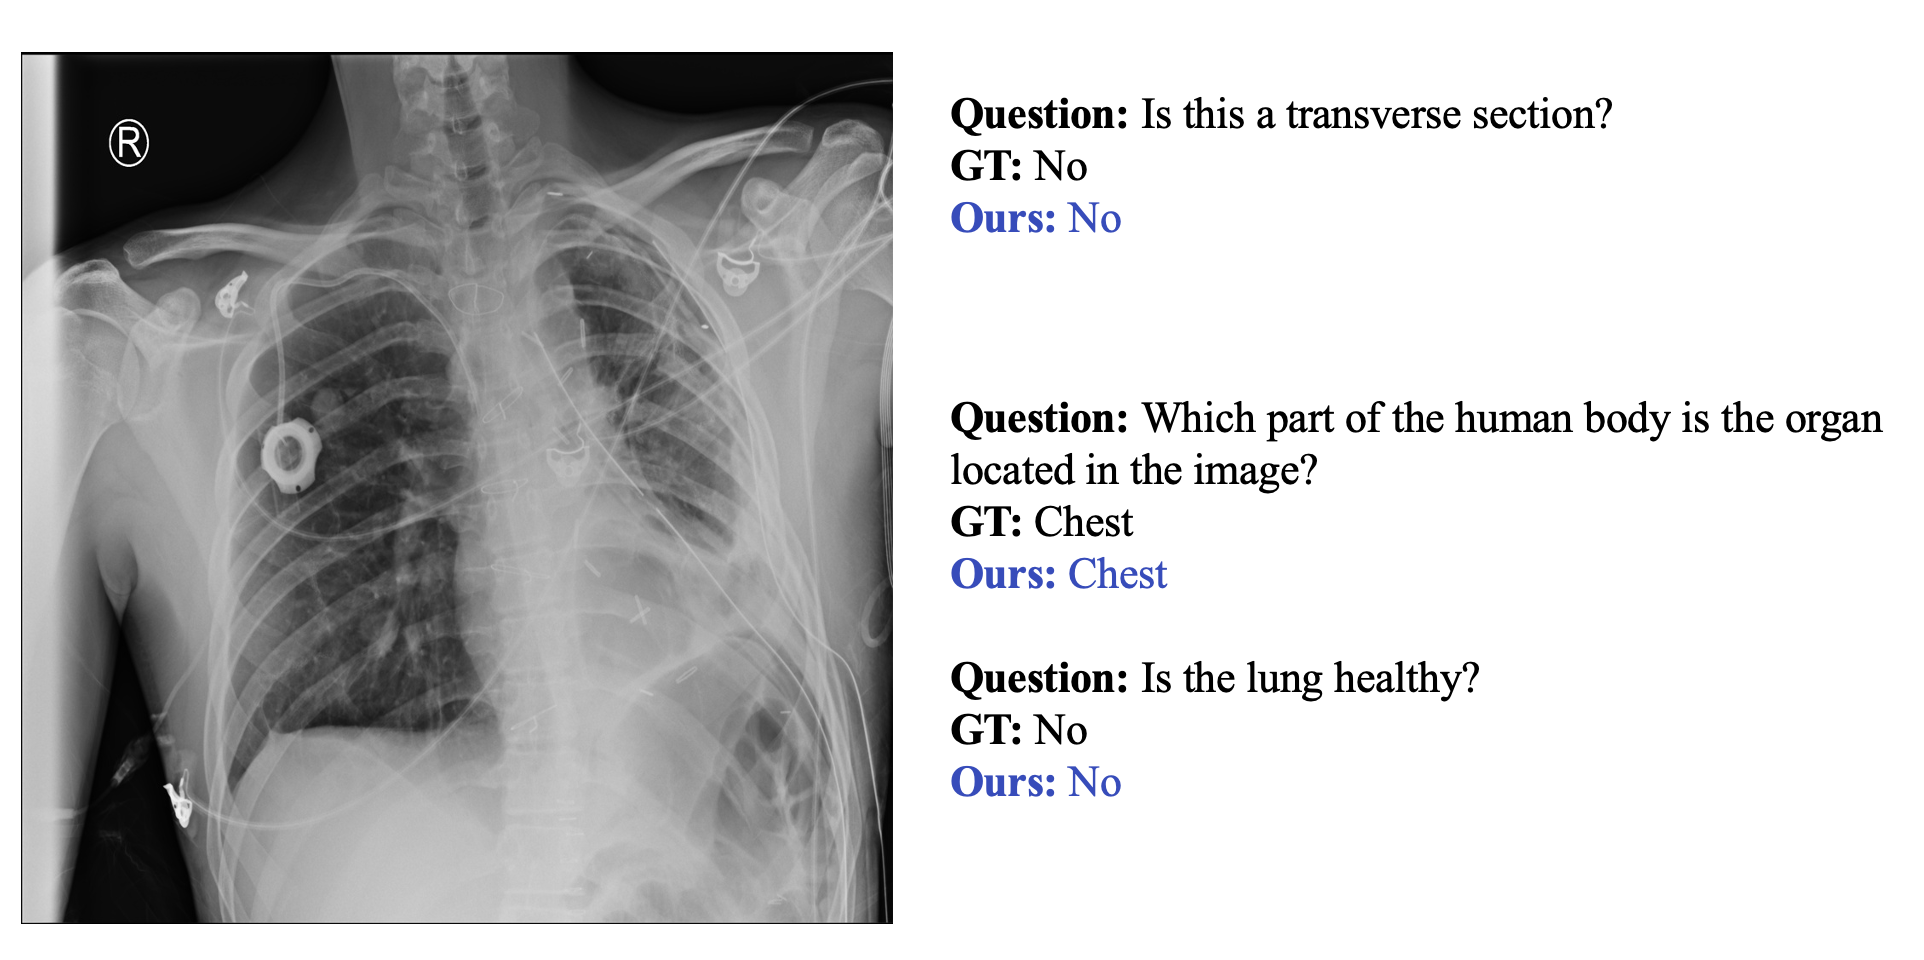
\includegraphics[width=1.0\linewidth]{Chapter_4/chap4_result5.png}
\end{center}
   \caption{Qualitative examples from our method on the SLAKE test splits.
}
\label{fig:qualitative5}
\end{figure}


\begin{figure}[t]
\begin{center}
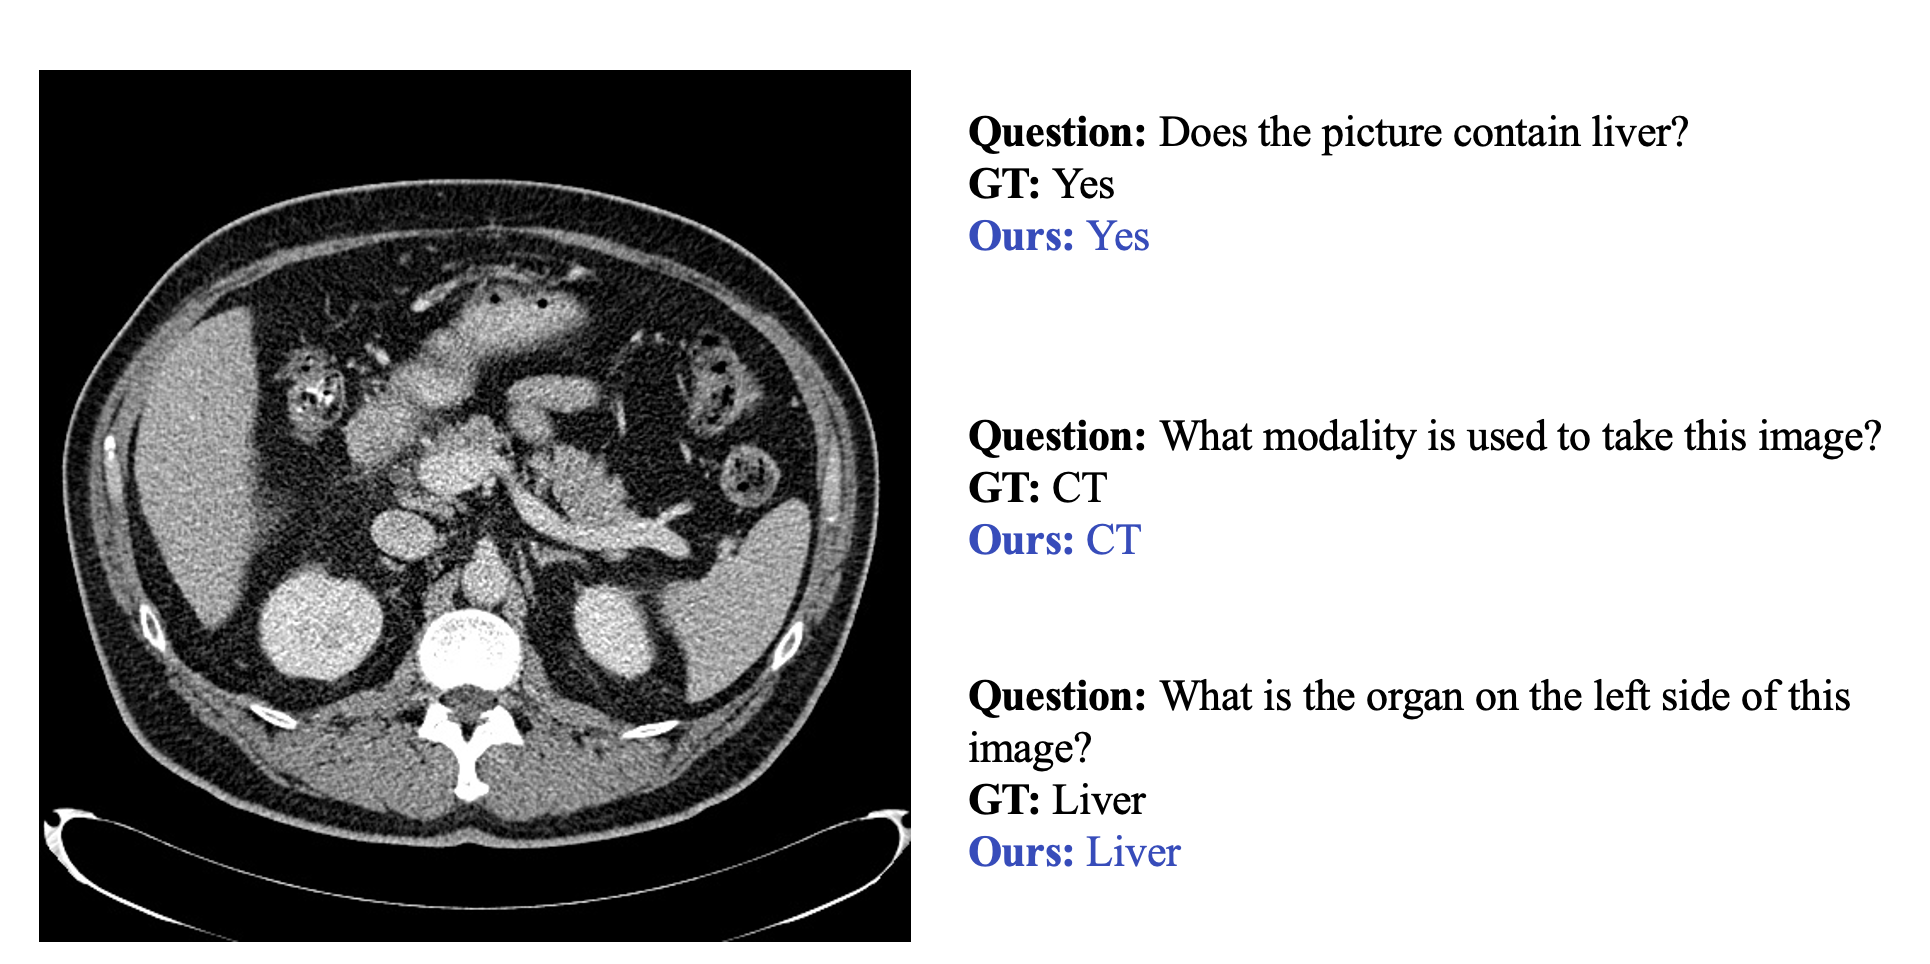
\includegraphics[width=1.0\linewidth]{Chapter_4/chap4_result6.png}
\end{center}
   \caption{Qualitative examples from our method on the SLAKE test splits.
}
\label{fig:qualitative6}
\end{figure}


\begin{figure}[t]
\begin{center}
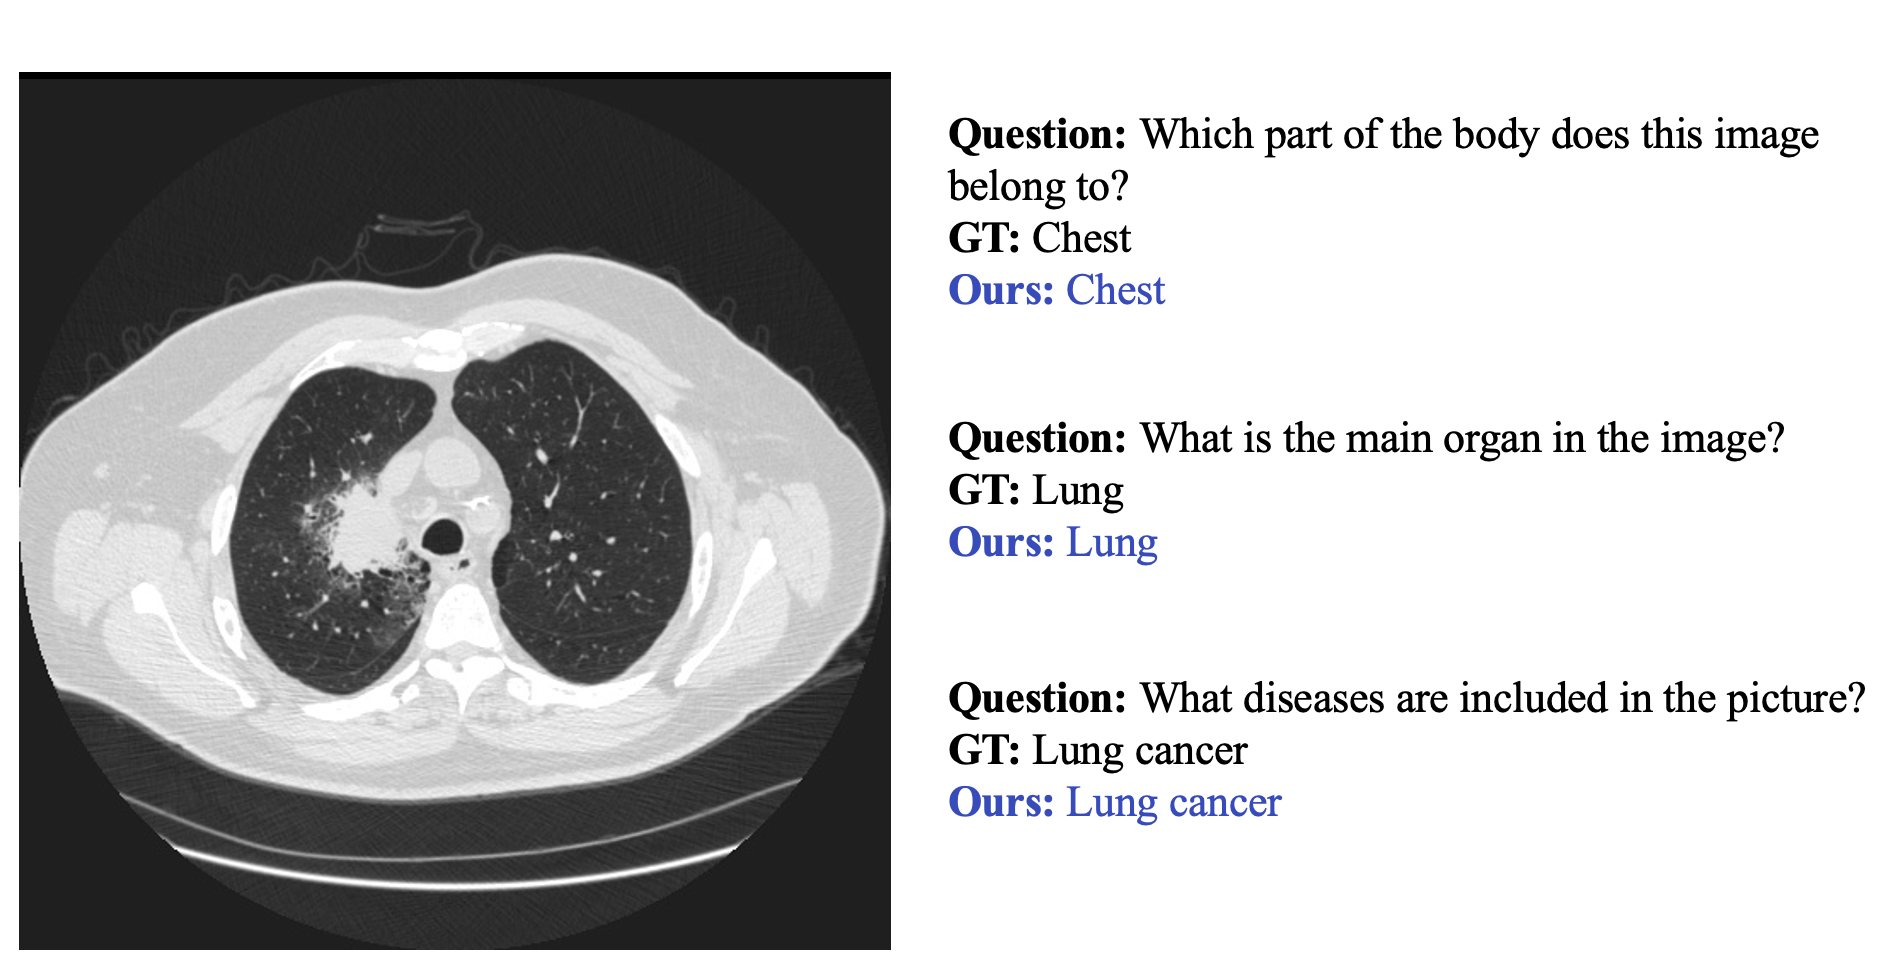
\includegraphics[width=1.0\linewidth]{Chapter_4/chap4_result7.png}
\end{center}
   \caption{Qualitative examples from our method on the SLAKE test splits.
}
\label{fig:qualitative7}
\end{figure}

\begin{figure}[t]
\begin{center}
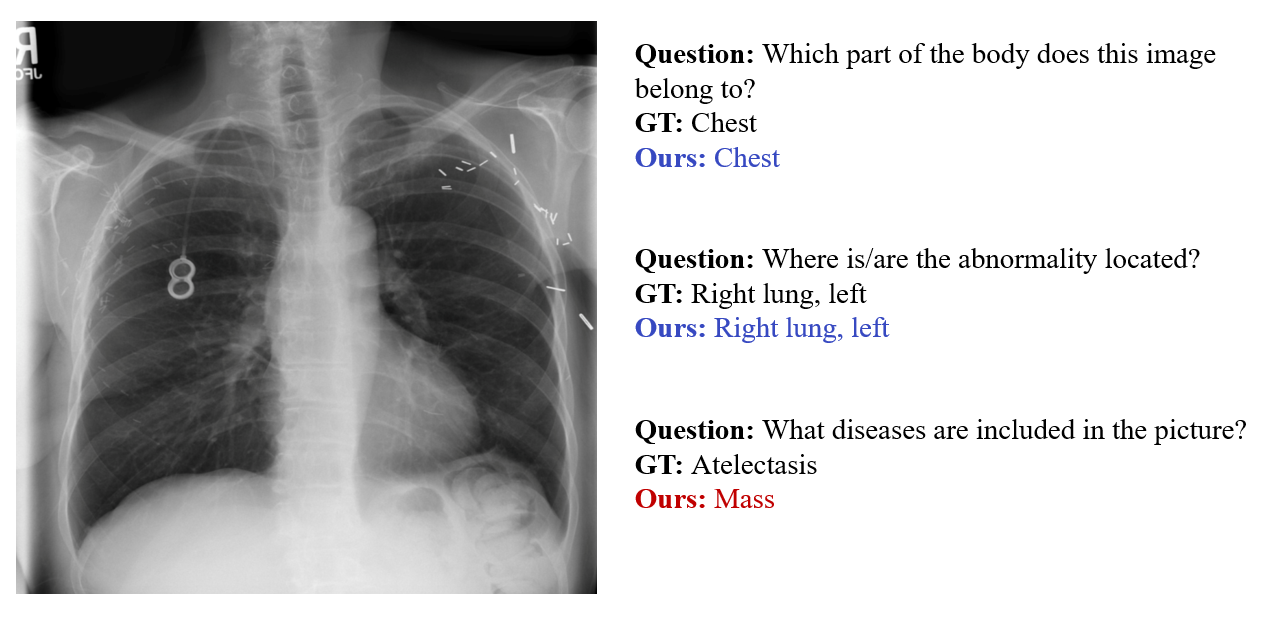
\includegraphics[width=1.0\linewidth]{Chapter_4/chap4_result2.png}
\end{center}
   \caption{Qualitative examples from our method on the SLAKE test splits. The red color highlights the failure cases.
}
\label{fig:qualitative2}
\end{figure}


\begin{figure}[t]
\begin{center}
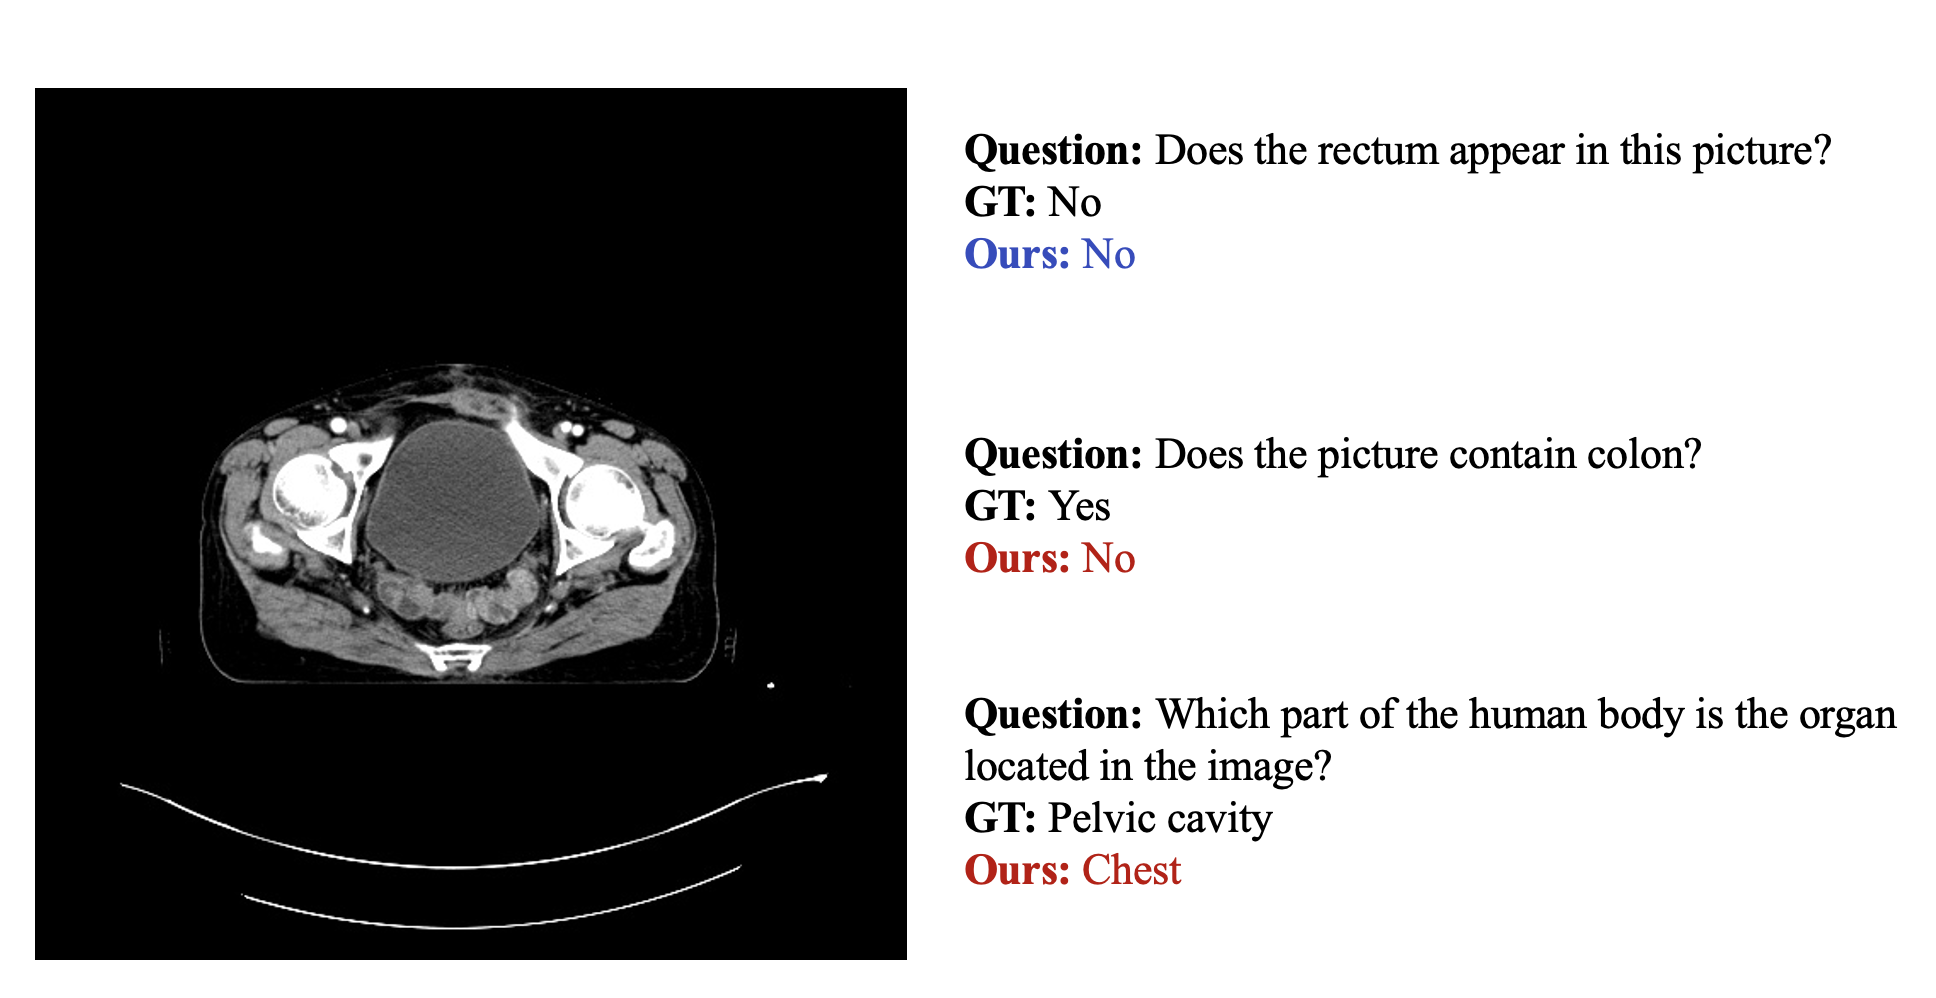
\includegraphics[width=1.0\linewidth]{Chapter_4/chap4_result8.png}
\end{center}
   \caption{Qualitative examples from our method on the SLAKE test splits. The red color highlights the failure cases.
}
\label{fig:qualitative8}
\end{figure}